\documentclass[nocopyrightspace,11pt,authoryear,preprint]{sigplanconf}

\usepackage{amsmath}
\usepackage{graphicx}
\usepackage{listings}
\renewcommand{\lstlistingname}{Code example}

%%% Syntax coloration
\usepackage{listings}
\usepackage{color}
\definecolor{lightgray}{rgb}{.9,.9,.9}
\definecolor{darkgray}{rgb}{.4,.4,.4}
\definecolor{purple}{rgb}{0.65, 0.12, 0.82}
\definecolor{ghostwhite}{RGB}{248, 248, 248}
\definecolor{brown}{RGB}{165, 42, 42}
\definecolor{violetred}{RGB}{186, 33, 39}
\definecolor{darkgreen}{RGB}{0, 128, 0}
\definecolor{comment}{RGB}{64, 128, 128}

\lstdefinelanguage{JavaScript}{
  keywords={typeof, new, for, true, false, catch, function, return, null, catch, switch, var, if, in, while, do, else, case, break, class, extends, super},
  keywordstyle=\color{darkgreen}\bfseries,
  ndkeywords={class, export, boolean, function, throw, implements, import, this},
  ndkeywordstyle=\color{darkgray}\bfseries,
  identifierstyle=\color{black},
  sensitive=false,
  comment=[l]{//},
  morecomment=[s]{/*}{*/},
  commentstyle=\color{comment}\ttfamily,
  stringstyle=\color{violetred}\ttfamily,
  morestring=[b]',
  morestring=[b]"
}

\lstset{
   language=JavaScript,
   backgroundcolor=\color{ghostwhite},
   extendedchars=true,
   basicstyle=\footnotesize\ttfamily,
   showstringspaces=false,
   showspaces=false,
   numbers=left,
   numberstyle=\footnotesize,
   numbersep=9pt,
   tabsize=2,
   breaklines=true,
   showtabs=false,
   captionpos=b
}

\usepackage{etoolbox}
\newtoggle{callstackdone}
% Is the callstack done?
\toggletrue{callstackdone}

\usepackage{hyperref}

\begin{document}
%% To import in the preambule
%\usepackage{listings}

% "define" Tool
\lstdefinelanguage{tool}{
  alsoletter={@},
  morekeywords={abstract, case, catch, class, def, do, else, extends, false, final, finally, for, if, implicit, import, match, new, null, object, 
override, package, private, protected, requires, return, sealed, super, this, throw, trait, try, true, type, val, var, while, with, yield, domain, 
postcondition, precondition, invariant, constraint, assert, forAll, in, _, return, @generator, ensure, require, ensuring },
  sensitive=true,
  morecomment=[l]{//},
  morecomment=[s]{/*}{*/},
  morestring=[b]"
}

\newcommand{\codestyle}{\small\sffamily}


% Default settings for code listings
\lstset{
  frame=tb,
  language=tool,
%  aboveskip=3mm,
%  belowskip=3mm,
%  lineskip=-0.1em,
  showstringspaces=false,
  columns=fullflexible,
  mathescape=true,
  numbers=none,
  numberstyle=\tiny,
  basicstyle=\codestyle
} 


\title{A Tool debugger in the browser}
\subtitle{Compiler Construction 2014 Final Report}

\authorinfo{Hadrien Milano\and Christophe Tafani-Dereeper}
           {EPFL}
           {\{hadrien.milano, christophe.tafani-dereeper\}@epfl.ch}

\maketitle

\section{Introduction}
During the semester, we have implemented a full compiler for Tool written in Scala. It outputs Java byte code which can consequently run on the JVM.

Throughout this period, we had the occasion to write quite a number of Tool programs, which allowed us to notice that it could be tedious to debug Tool code. That's why we chose to develop a debugger for Tool.

\subsection{Features}

\begin{enumerate}
\item Load Tool source files, or develop directly in the web IDE
\item Set breakpoints in the code
\item Step-by-step execution: step over lines, step into / out function calls
\item See the value of every variable
\item See the current call stack
\item integrated code editor and compiler
\end{enumerate}

We chose to implement our debugger as a single web page such that it is cross platform, easy to use (no binary to download) and can still be used offline. Moreover, it allows us to leverage the browser's garbage collector to implement easily the debugging VM (see "Virtual machine implementation")

\subsection{Running the debugger}

An online version of the debugger is available at the following URL : \href{http://bit.ly/tool-debugger}{bit.ly/tool-debugger}. It can also be run locally by opening the \textsc{index.html} file of the Git repository.

% [Describe in a few words what you did in the first part of the compiler project
%(the non-optional labs)]Lorem ipsum dolor sit amet, consectetur adipisicing elit, sed do eiusmod
%tempor incididunt ut labore et dolore magna aliqua. Ut enim ad minim veniam,
%quis nostrud exercitation ullamco laboris nisi ut aliquip ex ea commodo

%[and briefly say what problem you want to solve with
%your extension.] In the process of writing our compiler we faced major issues %for writing tool programs. Without a way to debug our tool programs, we can't %know for sure wether a given bug is due to our compiler or our program. We %therefore found it could be useful not only for us but also for future %iterations of this course to have a tool language debugger.

%This extension does not involve many modifications of the previously achieved %work but requires a bit of additionnal software.



%This section should convince us that you have a clear picture of the general
%architecture of your compiler and that you understand how your extension fits
%in it.


\section{Examples}
Give code examples where your extension is useful, and describe how they work
with it. Make sure you include examples where the most intricate features of
your extension are used, so that we have an immediate understanding of what the
challenges are.

You can pretty-print tool code like this:
\begin{lstlisting}
object {
  def main() : Unit = { println(new A().foo(-41)); }
}

class A {
  def foo(i : Int) : Int = {
    var j : Int;
    if(i < 0) { j = 0 - i; } else { j = i; }
    return j + 1;
  }
}
\end{lstlisting}

This section should convince us that you understand how your extension can be
useful and that you thought about the corner cases.


\section{Implementation}
This is a very important section, you explain to us how you made it work.

\subsection{Modifying the compiler backend}
\label{backend}

First, we had to make a new version of the code generator. The compiler now outputs a JSON file, containing the elements described below.

\begin{itemize}
\item The list of the classes that the program contains
\item For each class, the list of its methods
\item For each method
	\begin{itemize}
	\item the variables declared in it
	\item the arguments list, along with their type
	\item the code
	\end{itemize}
\end{itemize}

The code takes the form of a custom simplified bytecode-like language, whose full specification can be found in the Annex. It is similar to Java's, with several notable differences.

\begin{itemize}
\item variables, methods and classes are referred to by their name, and not a numeric identifier
\item an instruction \textsc{stat} is used to map bytecode instructions to source code lines
% todo
\end{itemize}


%If you are using theoretical concepts, explain them first in this subsection.
%Even if they come from the course (eg. lattices), try to explain the essential
%points \emph{in your own words}. Cite any reference work you used like this
%\cite{TigerBook}. This should convince us that you know the theory behind what
%you coded. 



\subsection{Porting the compiler in the browser}

To make the compiler run in the browser, we used \textsc{ScalaJS}, an EPFL-made library that transcompiles Scala to JavaScript.
\textbf{TODO[Hadrien] Talk about browserFS}
This allows us to conveniently output a JSON file (described in section \ref{subsec:backend}) containing the program structure and code.


\subsection{Implementation of the virtual machine}

At this stage, we have a compiler able to run in the browser and output a custom representation of any Tool program, but nothing to interpret it.
We have implemented a JavaScript virtual machine able to execute instructions that we have defined for our custom bytecode-like language.

\subsubsection{Architecture}

The execution is handled by the Engine class. It contains a StateMachine and methods to handle the debugging control flow (breakpoints, run, step into, etc.).
The state machine contains information about the current state of the program (stack, program counter, current scope...) as well as methods to change it.\\

\begin{figure}[h]
  \centering
    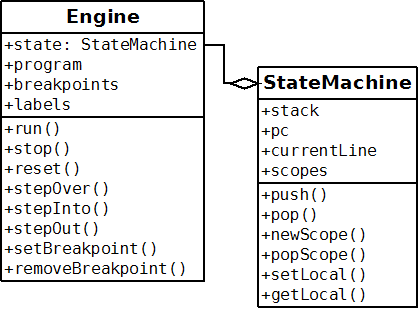
\includegraphics[scale=0.6]{diag.png}
     \caption{(Non-exhaustive) class structure}
\end{figure}

\subsubsection{Control flow}

\textbf{TODO : talk about labels, step in, step out, etc}

\subsection{Developing the web interface}

After that, we had to implement the web interface of the debugger. It is divided into four main parts.

\begin{itemize}
\item The code editor, where you can type code and set breakpoints
\item The toolbar, which allows you to load a Tool source file, compile it, and control the debugging process (run / stop / step over / step into / step out)
\item The console, where you can see messages from the debugger, compilation errors, and the program output
\item The right panel, that allows you to see the values of the variables in the current scope
\iftoggle{callstackdone}{%
	and the callstack
}{%
}.
\end{itemize}

The interface was made in HTML and JavaScript, with the use of \href{http://dojotoolkit.org/reference-guide/1.10/dijit/}{Dijit}, a popular library to create web user interfaces.

\subsection{Implementation Details}
Describe all non-obvious tricks you used. Tell us what you thought was hard and
why. If it took you time to figure out the solution to a problem, it probably
means it wasn't easy and you should definitely describe the solution in details
here. If you used what you think is a cool algorithm for some problem, tell us.
Do not however spend time describing trivial things (we what a tree traversal
is, for instance). 

After reading this section, we should be convinced that you knew what you were
doing when you wrote your extension, and that you put some extra consideration
for the harder parts.


\section{Possible Extensions}
We will use this section to discuss another implementation possibility as well as how we could improve our solution.

\paragraph{}
One of the things we were told is that we could have transpiled tool to javascript, generated a source map file and then used a native debugger such as the Chrome developper tools. While this approach may seem beneficial at first (we use a robust and full featured piece of GUI), it is limited and actually not suitable for our purpose. A source map is only a way to debug something that is meant to be run in a javascript environment. It depends on javascript's underlying types and does not allow a great deal of language-specific customization. \\On the other hand, we want the tool program to behave identically as in the JVM or anywhere else --- and this even when types are pushed to their limits. Also, our approach allows to integrate the compiler and the debugger in a coherent environment which is much more comfortable to use.

\paragraph{}
We are quite satisfied with the solution we came up with. We believe that with this tool (no pun intended), we would have gained massive time when writing test programs. The feedback loop of writing code, finding bugs, killing them and writing code again would have been much tighter with everything contained in one single interface. We acknowledge that it is far from being perfect and we have a few ideas of things that could have been further improved.

\begin{itemize}
\item The VM should run in a separate thread than the UI. This allows the interface to stay responsive even when the program is stucked. Currently, if a program loops indefinitely, the web page has to be closed. It is not a trivial modification and involves some work with HTML5 web workers and messaging --- we believe this was a little out of the scope of this extension.
\item Although the core software involved here works well, the UI is still pretty rough and could have been improved a bit. For instance, we could make the variables tree not to collapse each time we step over an instruction.
\item Some debugging related features could be added: watch the value of expressions, change the value of variables from the interface, set conditional breakpoints...
\end{itemize}

\bibliographystyle{abbrvnat}
\bibliography{bibliography.bib}

\end{document}
